%%%%%%%%%%%%%%%%%%%%%%%%%%%%%%%%%%%%%%%%%
% FRI Data Science_report LaTeX Template
% Version 1.0 (28/1/2020)
% 
% Jure Demšar (jure.demsar@fri.uni-lj.si)
%
% Based on MicromouseSymp article template by:
% Mathias Legrand (legrand.mathias@gmail.com) 
% With extensive modifications by:
% Antonio Valente (antonio.luis.valente@gmail.com)
%
% License:
% CC BY-NC-SA 3.0 (http://creativecommons.org/licenses/by-nc-sa/3.0/)
%
%%%%%%%%%%%%%%%%%%%%%%%%%%%%%%%%%%%%%%%%%


%----------------------------------------------------------------------------------------
%	PACKAGES AND OTHER DOCUMENT CONFIGURATIONS
%----------------------------------------------------------------------------------------
\documentclass[fleqn,moreauthors,10pt]{ds_report}
\usepackage[english]{babel}

\graphicspath{{fig/}}

\usepackage{graphicx}
\usepackage{subcaption}




%----------------------------------------------------------------------------------------
%	ARTICLE INFORMATION
%----------------------------------------------------------------------------------------

% Header
\JournalInfo{FRI Data Science Project Competition 2023}

% Interim or final report
% \Archive{Interim report} 
\Archive{Final report} 

% Article title
\PaperTitle{A Survey and Empirical Comparison of Synthetic Data Generation Methods for Relational Data} 

% Authors (student competitors) and their info
\Authors{Valter Hudovernik and Martin Jurkovič}

% Advisors
\affiliation{\textit{Advisor: prof. dr. Erik Štrumbelj}}

% Keywords
\Keywords{Synthetic data generation, relational data, synthetic data evaluation}
\newcommand{\keywordname}{Keywords}


%----------------------------------------------------------------------------------------
%	ABSTRACT
%----------------------------------------------------------------------------------------

\Abstract{
% Synthetic relational data generation has gained significant attention in academia and industry. We conduct a comprehensive overview of the field, benchmarking available methods and contributing to the evaluation process. Our research focuses on evaluating synthetic tabular relational data using a specially designed benchmark that incorporates four standard datasets and five state-of-the-art methods. Through rigorous empirical analysis we identify the most effective method, which we apply to generate synthetic data for Zurich Insurance Group. Our findings contribute to advancing the field by providing valuable insights and examining potential use cases for our industry partner.
Synthetic relational data generation has gained significant attention in academia and industry. We conducted a comprehensive overview of the field, benchmarking available methods and contributing to the evaluation process. Our research focuses on evaluating synthetic tabular relational data using a specially designed benchmark that incorporates four standard datasets and five state-of-the-art methods. Through rigorous empirical analysis we evaluated all of the methods, which we then applied to generate synthetic data for Zurich Insurance Group. Our findings contribute to the advancement of the relational data generation field by providing valuable insights and examining potential use cases for our industry partner.
}

%----------------------------------------------------------------------------------------

\begin{document}

% Makes all text pages the same height
\flushbottom 

% Print the title and abstract box
\maketitle 
% Removes page numbering from the first page
\thispagestyle{empty} 

%----------------------------------------------------------------------------------------
%	ARTICLE CONTENTS
%----------------------------------------------------------------------------------------

\section{Introduction}
We were motivated by Zurich Insurance Group (ZI) to research the field of synthetic data generation methods that support relational data. We found 7 methods, including 2 commercial tools, which we describe in Section \ref{sec:relational}. 

There is no comprehensive evaluation of the quality of these methods and as such, users have little information on which method is best and what their limitations are. We contribute to the field by conducting the first comprehensive empirical evaluation and comparison.

Synthetic relational data impacts healthcare and financial fields the most, so it is also relevant for insurance companies such as our industry partner ZI. It promises several benefits, ensuring privacy by generating artificial data, and safeguarding sensitive information, which is crucial in the insurance business. Additionally, synthetic data generation is cost-effective and time-efficient, making it advantageous for quick iteration and prototyping in time-sensitive situations. Moreover, synthetic data provides additional data points alleviating issues like class imbalance and impurities.

Methods for tabular data generation have seen numerous advancements in the recent years and received significant attention~\cite{Borisov_2022}. Generating realistic tabular data is a challenging task due to complex interdependencies, diverse data distributions, data irregularities, domain-specific constraints and evaluation difficulties. Tabular data contains intricate relationships between columns, requires replicating statistical properties accurately, handling missing values and outliers and ensuring adherence to domain constraints. Evaluating the realism of generated data adds another layer of complexity. Recently the work of Zein and Urvoy ~\cite{zein2022tabular} showcases that using discriminative models can highlight the discrepancies between real and generated data and sheds a light on the shortcomings of established evaluation procedures.

Synthesizing relational databases poses additional challenges to tabular data synthesis as it also requires modeling the relationships between tables. 

These relationships introduce new non-trivial constraints and dependencies that generative models must address in order to effectively generate synthetic data.

\section{Relational Data Generation} \label{sec:relational}
 \subsection{Methods}

\textbf{The Synthetic data vault} by Patki et al. (2016)~\cite{SDV} introduced the first method for relational synthetic data generation. They proposed a recursive conditional parameter aggregation technique to model tables in a relational database. They focus on privacy protection and demonstrating the utility of synthetic data. To generate the data, users are required to specify the metadata or structure of the data, which has since become a common practice in the field.

Gueye et al. (2022) proposed the \textbf{Row Conditional-TGAN (RC-TGAN)}~\cite{RC-TGAN}, an extension of the tabular GAN model to relational data. RC-TGAN incorporates conditional data from parent rows into the child table GAN model, allowing it to handle various relationship schemas without additional processing. Additionally, they enhance RC-TGAN to capture the influence of grandparent rows on their grandchild rows, preserving this connection even when the relationship information is not transferred by the parent table rows.

 \textbf{Realistic Relational and Tabular Transformer (REaLTabFormer)} by Solatorio and Dupriez (2023) \cite{solatorio2023realtabformer} is a synthetic data generation model based on GPT-2. The model focuses on generating single parent relational data and employs a GPT-2 encoder with a causal language model (LM) head to independently model the parent table. The encoder is frozen after training and used to conditionally model the child tables. Each child table requires a new conditional model, implemented as a sequence-to-sequence (Seq2Seq) transformer. The GPT-2 decoder with a causal LM head is trained to generate observations from the child table, accommodating variable lengths.

Additionally we evaluated commercial tools for synthetic data generation. Two of them stand out for their support of relational data generation. \textbf{MostlyAI} (\url{https://mostly.ai}) does not disclose the specific generative model used during data generation. \textbf{GretelAI} (\url{https://gretel.ai}) employs a tabular LSTM model for generating synthetic samples. Both tools incorporate privacy checks and data filtering mechanisms as part of their process.

We list also the work of Mami et al. \cite{mami2022generating}, using Graph Variational Auto Encoders, and Canale et al. \cite{canale2022generative}, which outline a framework for synthetic relational data generation using causal transformers. No API or source is available for these methods, but this will hopefully change after our correspondence with the authors.

\subsection{Evaluation Metrics}
Common single-table metrics are statistical tests on column distributions, such as the Kolmogorov-Smirnov test, Jensen-Shannon distance, Chi-squared test and Maximum Mean Discrepancy. The most common relational data metrics are Logistic Detection (LD) and Machine Learning Efficacy (ML-E). LD employs a Logistic Regression Classifier to discriminate between synthetic and real data. It is calculated for each table in the hierarchical dataset by comparing it to its corresponding synthetic counterpart. 

To evaluate the generative model's ability to preserve parent-child relationships, an extended version of LD known as parent-child logistic detection (P-C LD) is utilized. P-C LD applies LD to denormalized synthetic tables, assessing the preservation of parent-child associations. A major drawback of LD is its inability to capture interactions between columns, so it is unable to discriminate between real and synthetic data when the synthetic data generate marginal distributions well. Figure~\ref{fig:univariate} illustrates how well state-of-the-art methods can match marginal distributions.

\begin{figure}[h!]
    \centering
    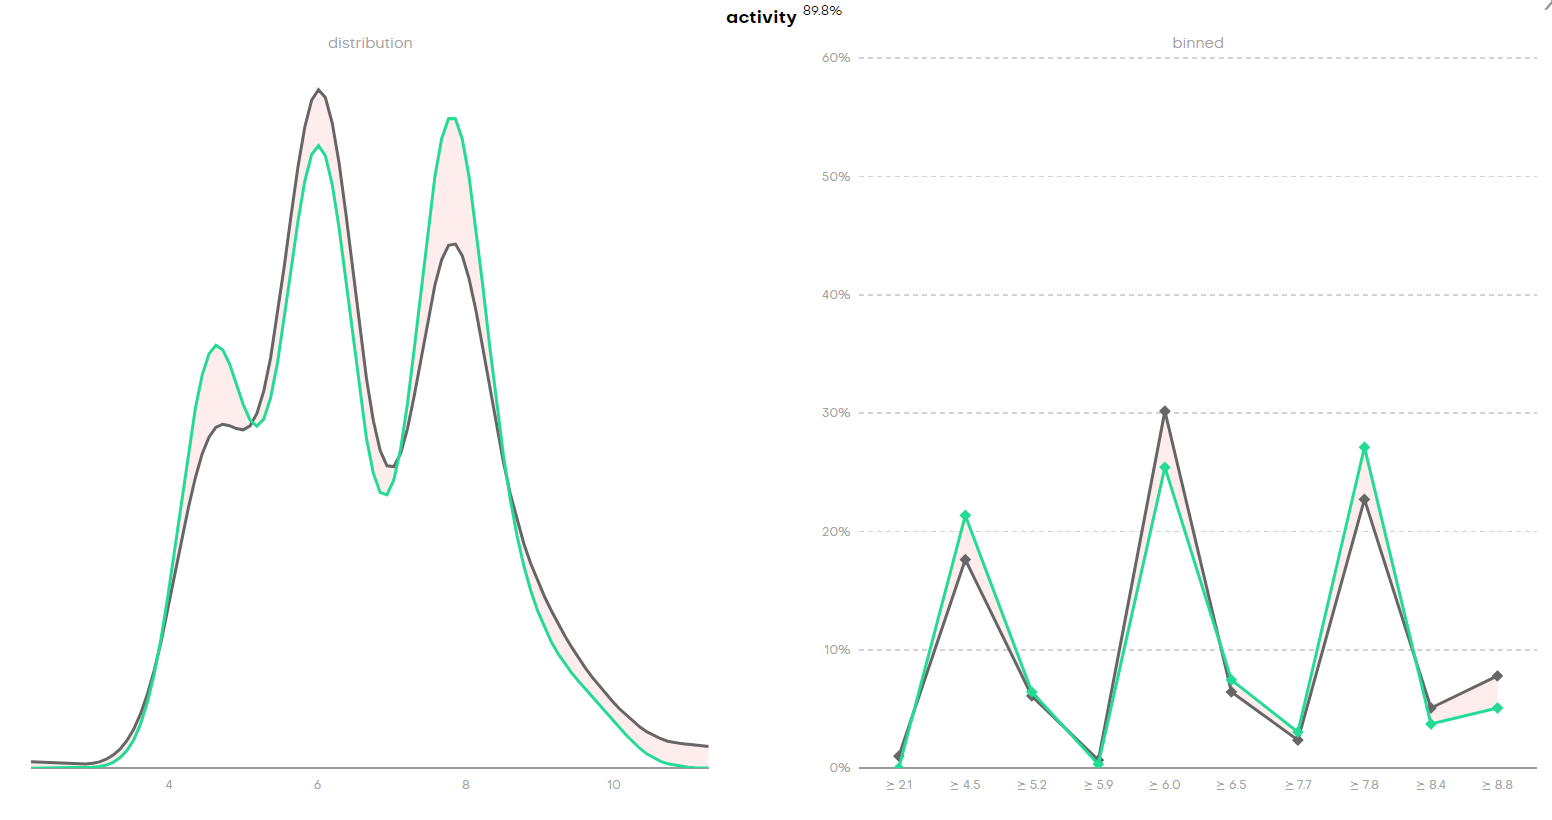
\includegraphics[width=\linewidth]{fig/mostly-univariate.png}
    \caption{\textbf{Univariate fits by Mostlyai on the biodegradability molecule table} show how well the methods are able to model even complex distributions.
    }
    \label{fig:univariate}
\end{figure}

ML-Efficacy compares the performance of the ML models for a specific task after training them on original vs. synthetic data and evaluating them on the test set of the original data. 
While this method provides good insight into the application of synthetic data, it is specific to the machine learning task, feature engineering and model. While this is a commonly used method for synthetic tabular and relational data evaluation we note that it does not describe the authenticity of the generated data other than capturing the task specific patterns.

\subsection{Evaluation Datasets}
We include four datasets that are widely used in related work: Rossmann Store Sales~\cite{rossmann_kaggle}, Biodegradability~\cite{biodegradability}, Mutagenesis~\cite{mutagenesis} and the Telstra Competition dataset~\cite{telstra_kaggle}. We also include data provided by ZI, a hierarchical historical customer data on customers, their policies and claims.

\section{Evaluation procedure}
We present a novel evaluation procedure based on k-fold cross-validation (k = 10 for our experiments) for both data generation and evaluation. Each dataset is partitioned into k folds by sampling at random from the parent table, then we use a hierarchical conditional sampling approach for the child tables. 

For single-column analysis we use the two-sample KS test, JS divergence, Maximum Mean Discrepancy and the Chi-squared test. Next, we use LD and P-C LD as an approach that also takes into account inter-column and inter-table interactions. We evaluate P-C LD on a denormalized table which combines the root table with the child columns. Despite breaking the IID assumption for our discrimination task, this approach results in better discrimination compared to single-table methods. Note that LD is used by all referenced related work.

Our first contribution to the evaluation process of relational generation methods is to include models that can model interactions and non-linearities (for this work, XGBoost). Our second contribution is to enriching the parent table with features derived from child tables while maintaining the IID assumption. In this work we (a) add counts of child rows for each table as well as the counts and means of grandchild tables and (b) add column means of the numeric columns in the child table. We showcase the improvements of using XGBoost over logistic regression and additional improvements by adding the aggregated information in Figure~\ref{fig:discriminative-detection-all}.

%------------------------------------------------

\section{Results}

In the results we include an idealized method that generates synthetic data by sampling from original data. It serves as a baseline for comparison and as validation of the evaluation metrics - it should pass all the tests and models should not be able to discriminate between real data and resampled real data generated by the method.

\subsection{Statistical Tests}
\begin{table}[!ht]
\centering
\resizebox{\columnwidth}{!}{
    \begin{tabular}{| l | l | l | l | l |}
    \hline
      Method & KS & JS &  MMD & $\chi^2$ \\
      \hline			 
      Baseline       & $.87\pm.01$ & $.17\pm.01$ &  $.12	\pm.01$ & $.55\pm.02$  \\
      \hline		
      REaLTabF  &  $.86\pm.01$  & $.17\pm.01$ &  $.08\pm.01$  &  $.49\pm.02$\\
      SDV           & $.78\pm.01$ &  $.23\pm.01$ & $.12\pm.01$  &  $.38\pm.02$ \\
      RCTGAN    &  $.80\pm.01$  & $.20\pm.01$ &$.29\pm.03$ & $.38\pm.02$\\
      Mostlyai        &  $.86\pm.01$  &  $.18\pm.01$ &  $.13\pm.01$ & $.51\pm.02$\\
      Gretel       &  $.86\pm.01$  & $.17\pm.01$ & $.21\pm.02$ & $.60\pm.05$\\
      \hline
    \end{tabular}
    }
    \caption{\textbf{Statistical test results on the root table of the Rossmann dataset.} We report the cross-validation means and standard erros of the Kolmogorv-Smirnov test (KS), Jensen-Shannon distance (JS), Maximum Mean Discrepancy (MMD) and Chi-squared test. We omit the leading zeros.}
    \label{tab:statistical}
\end{table}

The averaged statistical test results for the root table of the Rossmann Store Sales dataset are shown in Table \ref{tab:statistical}. The Store table contains categorical and numerical columns and these results are a representative example of results for other datasets. We find that these statistical tests do not effectively differentiate between the evaluated methods, because methods model marginal distributions well, which can also be seen in Figure~\ref{fig:univariate}.


\subsection{Discriminative Detection}

This discrimination capability of XGBoost is illustrated in Figure~\ref{fig:discriminative-detection-all}. Even though we do not get perfect instance-level discrimination for every experiment, the classification accuracies are high enough so that we would with perfect accuracy be able to identify a synthetic dataset\footnote{Comparative visualizations for all datasets and tables are available at \url{https://github.com/martinjurkovic/Synthetic-data-generation-project/blob/master/RESULTS.md}}. 

\begin{figure}[h!]
\centering
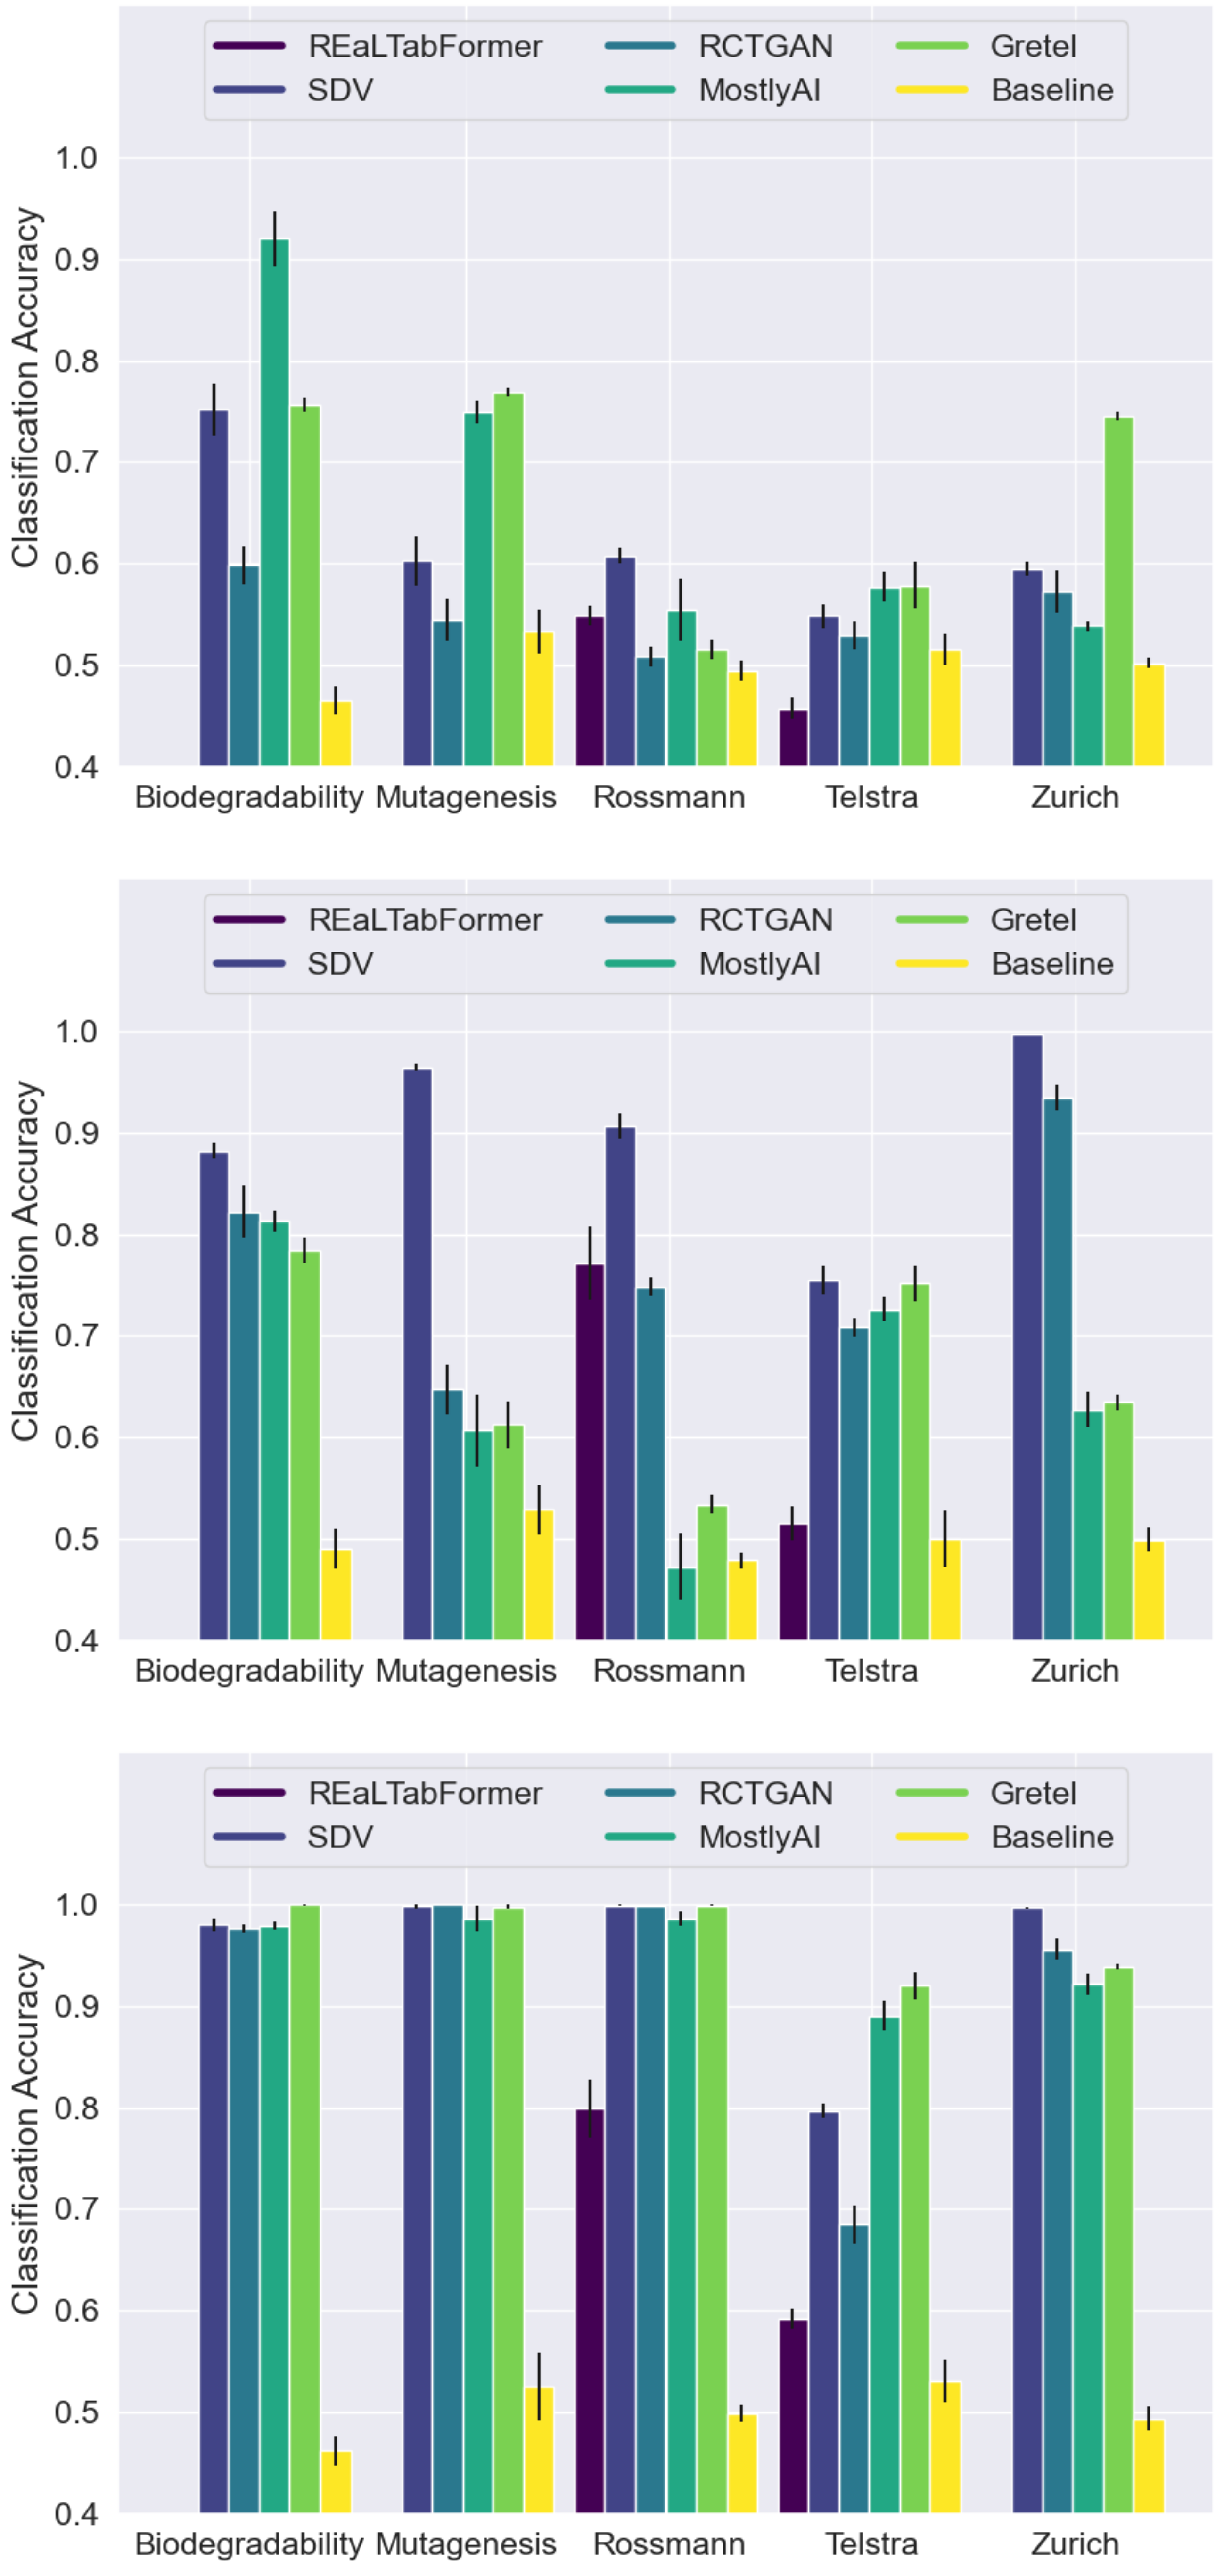
\includegraphics[width=\linewidth]{fig/all_datasets_log_xgb_child.png}
\caption{\textbf{Logistic detection (top) vs. XGB detection (middle) vs. XGB with child count and child column means (bottom) on denormalized datasets.} Our method is able to almost perfectly distinguish between original and synthetic data rows for every dataset and method except REaLTabFormer, which is only calculated for Rossman Store Sales and Telstra Competition as it can only generate one level of children. Worse results overall on the Telstra dataset can be explained by the fact that the data can be denormalized well into a single table because the children only have one column and it is a trivial relational database.}
\label{fig:discriminative-detection-all}
\end{figure}

\subsection{Machine Learning Efficacy}
GretelAI's study in ML-E for single table datasets for their method found that synthetic data average accuracy with no Privacy Filters is usually not far from the original data’s average accuracy~\cite{steier2022gretel}. We achieved similar results while predicting fault severity for the Telstra dataset for all of the methods.

\begin{table}[h!]
\centering
\begin{tabular}{|l|r|r|r|}
\hline
Method & Accuracy & Precision & Recall \\
\hline
Original data & 0.89 & 0.77 & 0.44 \\
\hline
SDV & 0.84 & 0.09 & 0.01 \\
RCTGAN & 0.85 & 0.19 & 0.00 \\
MostlyAI & 0.22 & 0.15 & 0.93 \\
GretelAI & 0.85 & 0.49 & 0.29 \\
\hline
\end{tabular}
\caption{\textbf{Comparison of synthetic data generation methods as a train set for churn prediction.} Since majority classifier is 0.85 we see that with synthetic data the model was not able to outperform it. } 
\label{tab:ML-E-zurich}
\end{table}

For ML-E on the ZI dataset we combined efforts with the team of Drab Ž., Kastelec E. and Kogovšek Ž. who developed a churn prediction pipeline for ZI data. They provided us a train split of all tables in the ZI's dataset which we used to generate synthetic data with all of the eligible methods. Then they used the synthetic data to train their churn prediction models. In Table~\ref{tab:ML-E-zurich} we see that churn prediction using synthetic data is not able to outperform the majority class baseline. We believe the reason is synthetic datasets were not able to model the relationships between parent and child tables well because ZI's dataset has time series data.

\subsection{Privacy Metrics}

In addition to evaluating data fidelity and utility, privacy metrics were considered. While our focus was primarily on data quality we also assessed privacy preservation aspects, particularly the Nearest Neighbour Ratio (NNR) and Distance to Closest Record (DCR) metrics. Notably, RCTGAN was the only method that exhibited small amounts of potentially copied rows. It is the only one of the methods to not explicitly perform privacy filtering during sampling. This shows that implementing simple filtering procedures can prevent private information leakage in synthetic data.

%------------------------------------------------

\section{Discussion}
We make several contributions to the field of synthetic relational data generation.
\vspace{-0.2cm}
\begin{itemize}
\setlength\itemsep{0.1em}
\item The first comprehensive review of related work (methods and metrics) with a thorough empirical comparison.
\item A novel process for evaluation.
\item Insight into the shortcomings of typically used metrics and improvements in the form of using more expressive discrimination models and additional engineered child table features.
\item Empirical evidence that none of the methods are able to generate synthetic relational data that is indistinguishable from real data.
\end{itemize}

Our work is available as a Python package, accessible for evaluation of any data generation method (\url{https://github.com/martinjurkovic/synthetic-data-generation-project}).

Future work includes exploring discriminative model explanation to gain insights into the differences between synthetic and original data. We aim to create a widely available Python package along with establishing an interface and testing protocol for evaluating the generational capabilities of new methods.


%------------------------------------------------

\section*{Acknowledgments}
We thank our industry partner ZCAM for providing us with the idea, data and help during this project.


%----------------------------------------------------------------------------------------
%	REFERENCE LIST
%----------------------------------------------------------------------------------------
\bibliographystyle{unsrt}
\bibliography{report}


\end{document}